\documentclass{article}
%----------------------------------------------------------------------
\usepackage[polish]{babel}
\usepackage[utf8]{inputenc}
\usepackage[T1]{fontenc}
\usepackage[a4paper,top=2cm,bottom=2cm,left=3cm,right=3cm,marginparwidth=1.75cm]{geometry}
\usepackage{lmodern}
\usepackage{microtype}
\usepackage{amsmath,amssymb}
\usepackage{graphicx}
\usepackage{listings}
\usepackage{etoolbox}
\usepackage{booktabs}
\usepackage{algorithm}
\usepackage[noend]{algpseudocode}
\usepackage{tabularx}
\usepackage{array}
\usepackage{enumitem}
\usepackage[colorlinks=true, linkcolor=black, urlcolor=black, citecolor=black]{hyperref}
\usepackage{csquotes}
\usepackage[backend=biber,style=numeric,sorting=none,maxbibnames=4]{biblatex}
\addbibresource{references.bib}
\usepackage{subcaption}
\usepackage{xcolor}
\usepackage{float}
\usepackage{newfloat}
\usepackage{fancyvrb}
\usepackage{multirow}
\usepackage{siunitx}

% Liczby po polsku: przecinek dziesiętny, spójniki i półpauza w listach i zakresach
\sisetup{
    output-decimal-marker = {,},
    exponent-product = \cdot,
    group-separator = {\,},
    group-minimum-digits = 5,
    uncertainty-mode = separate,
    list-separator = {,~},
    list-pair-separator = {~i~},
    list-final-separator = {~i~},
    range-phrase = {--},
    range-units = single,
}
% Procent bez odstępu, jak na wykresach (94,1%)
\DeclareSIUnit[quantity-product = {}]\percent{\%}

% Wykresy brane wprost z katalogów eksperymentów i badań
\graphicspath{{../data/experiments/}}

% Definicje kolorów
\definecolor{consoleGreen}{RGB}{22, 198, 12}
\definecolor{consoleRed}{RGB}{197, 15, 31}
\definecolor{consoleYellow}{RGB}{193, 156, 0}
\definecolor{consoleBlue}{RGB}{0, 55, 218}
\definecolor{consoleGray}{RGB}{100, 100, 100}
\definecolor{consolePurple}{RGB}{136, 23, 152}

% Pomocnicze komendy do kolorowania
\newcommand{\txtGreen}[1]{\textcolor{consoleGreen}{#1}}
\newcommand{\txtRed}[1]{\textcolor{consoleRed}{#1}}
\newcommand{\txtYellow}[1]{\textcolor{consoleYellow}{#1}}
\newcommand{\txtBlue}[1]{\textcolor{consoleBlue}{#1}}
\newcommand{\txtGray}[1]{\textcolor{consoleGray}{#1}}
\newcommand{\txtPurple}[1]{\textcolor{consolePurple}{#1}}

\newfloat{code}{H}{loc}[section]
\floatname{code}{Listing}

% Algorytmy po polsku
\floatname{algorithm}{Algorytm}
\renewcommand{\algorithmicrequire}{\textbf{Wejście:}}
\renewcommand{\algorithmicensure}{\textbf{Wyjście:}}

% Oznaczenia używane w tekście
\newcommand{\yhat}{\hat{y}}
\newcommand{\RCS}{RCS}

\emergencystretch=1.5em

% Sekcje zaczynają się od nowej strony, dopóki nie wyłączymy tego przez \sekcjebezpodzialu
\newif\ifsekcjanowastrona
\sekcjanowastronatrue
\newcommand{\sekcjebezpodzialu}{\sekcjanowastronafalse}
\pretocmd{\section}{\ifsekcjanowastrona\clearpage\fi}{}{}

\lstset{
    basicstyle=\ttfamily, % Ustawienie czcionki monospaced
}

\newcommand{\nazwaprzedmiotu}{Sieci neuronowe}
\newcommand{\tytulprojektu}{Klasyfikacja i regresja z użyciem perceptronu wielowarstwowego}
\newcommand{\nazwadokumentu}{Raport}
\newcommand{\prowadzacy}{dr inż. Maksymilian Bujok \\ mgr inż. Grzegorz Zakrzewski}
%----------------------------------------------------------------------
\begin{document}

\begin{titlepage}
    \centering
    \vspace{1.5cm}
    
\includegraphics[width=0.9\textwidth]{university-logo.png} \\
    \vspace{2.5cm}
    {\fontsize{30}{20}\selectfont \textbf{\nazwaprzedmiotu} \par}
    \vspace{1.5cm}
    {\fontsize{25}{20}\selectfont \tytulprojektu \par}
    \vspace{1.5cm}
    {\fontsize{18}{20}\selectfont \nazwadokumentu \par}
    \vspace{1.5cm}
    {\fontsize{12}{20}\selectfont Zespół: \\ Adam Grącikowski \par}
    \vspace{0.5cm}
    {\fontsize{12}{20}\selectfont Prowadzący: \\ \prowadzacy \par}
    
    \vfill
    Oświadczam, że niniejsza praca, stanowiąca podstawę do uznania osiągnięcia efektów uczenia się z przedmiotu \textit{\nazwaprzedmiotu}, została wykonana samodzielnie. 

    \vspace{1cm}
    
    Warszawa, \today
    
\end{titlepage}

%----------------------------------------------------------------------
\section*{Streszczenie}
\phantomsection
\label{sec:abstract}

W projekcie zaimplementowano od podstaw, bez bibliotek sieci neuronowych, perceptron wielowarstwowy uczony propagacją wsteczną błędu i zbadano go w zadaniach regresji funkcji jednej zmiennej i klasyfikacji punktów płaszczyzny.

Na czterech zbiorach danych, w czterech licznościach zbioru uczącego, zbadano wpływ funkcji aktywacji, architektury sieci i funkcji straty. Każdy wariant uczono dla $10$ ziaren generatora liczb losowych, łącznie w \num{2400} eksperymentach, a wyniki porównywano na podstawie statystyk po ziarnach.

W klasyfikacji dla klas rozdzielonych prostą wystarczyła sieć bez warstw ukrytych, a dla nakładających się skupisk wystarczała jedna mała warstwa ukryta. Duże sieci uczone na małych zbiorach przeuczały się, a ich dokładność na zbiorze uczącym przewyższała testową nawet o \num{8.19} punktu procentowego. Funkcje aktywacji i funkcje straty dawały w klasyfikacji różnice rzędu dziesiątych części punktu procentowego.

W regresji błąd poza zakresem danych uczących zależał od kształtu przedłużenia funkcji sieci: dla funkcji o kształcie nasycającym sieć z funkcją tanh miała medianę MSE od \num{0.600} do \num{2.33}, a sieci z ReLU i leaky ReLU od \num{1410} do \num{2200}.

Wybór najlepszego wariantu na podstawie jednego ziarna różnił się od wyboru na podstawie $10$ ziaren w \qty{38}{\percent} przypadków w klasyfikacji i \qty{39}{\percent} w regresji, co potwierdza potrzebę uczenia każdego wariantu wielokrotnie.


\tableofcontents
\newpage

%----------------------------------------------------------------------
\section{Wstęp}
\label{sec:introduction}

\subsection{Cel i zakres projektu}
\label{sec:introduction-goal}
% Plan (etap 11): perceptron wielowarstwowy zaimplementowany od podstaw, bez bibliotek
% sieci neuronowych; regresja f: R -> R i klasyfikacja wektorów w R^2; wymagane
% wizualizacje i badania.

\subsection{Struktura raportu}
\label{sec:introduction-outline}
% Plan (etap 11): krótki przegląd rozdziałów z odwołaniami \ref.

\section{Opis problemu}
\label{sec:problem}

W rozdziale opisano dwa rozwiązywane zadania, sposób oceny ich rozwiązań, dostarczone zbiory danych oraz zakres badań wymagany w projekcie.

\subsection{Regresja i klasyfikacja}
\label{sec:problem-tasks}

Oba zadania należą do uczenia nadzorowanego (ang. \textit{supervised learning}). Dany jest zbiór uczący $\{(\mathbf{x}_i, y_i)\}_{i=1}^{n}$ par wejście-odpowiedź, na podstawie którego dobierane są parametry modelu. Celem nie jest jednak odtworzenie odpowiedzi ze zbioru uczącego, lecz poprawne przewidywanie dla nowych wejść. Dlatego jakość modelu ocenia się na osobnym zbiorze testowym, który nie jest używany w trakcie uczenia \cite{goodfellow2016}.

W zadaniu regresji wejściem jest liczba rzeczywista $x \in \mathbb{R}$, a odpowiedzią wartość $y \in \mathbb{R}$ pewnej nieznanej funkcji $f \colon \mathbb{R} \to \mathbb{R}$. Model zwraca przybliżenie $\yhat_i$ wartości $y_i$. Miarą jakości jest błąd średniokwadratowy (ang. \textit{mean squared error}, MSE) liczony na $m$ próbkach zbioru testowego w oryginalnej skali odpowiedzi:
\begin{equation}
    \mathrm{MSE} = \frac{1}{m} \sum_{i=1}^{m} \left( \yhat_i - y_i \right)^2 .
    \label{eq:mse}
\end{equation}

W zadaniu klasyfikacji wejściem jest wektor $\mathbf{x} \in \mathbb{R}^2$, a odpowiedzią numer klasy $y \in \{1, \dots, K\}$. Model zwraca rozkład prawdopodobieństwa na $K$ klasach, a decyzją $\yhat_i$ jest klasa o największym prawdopodobieństwie. Miarą jakości jest dokładność (ang. \textit{accuracy}), czyli odsetek poprawnie sklasyfikowanych próbek zbioru testowego:
\begin{equation}
    \mathrm{ACC} = \frac{1}{m} \sum_{i=1}^{m} \mathbf{1}\left[ \yhat_i = y_i \right] ,
    \label{eq:accuracy}
\end{equation}
gdzie $\mathbf{1}[\cdot]$ przyjmuje wartość $1$, gdy warunek jest spełniony, i $0$ w przeciwnym razie. Jeśli rozkłady klas nachodzą na siebie, w części przestrzeni wejść ta sama wartość $\mathbf{x}$ może należeć do różnych klas. Nawet optymalny klasyfikator, zwany klasyfikatorem Bayesa, myli się wtedy na części próbek, więc dokładność \qty{100}{\percent} jest nieosiągalna \cite{bishop2006}.

Miary \eqref{eq:mse} i \eqref{eq:accuracy} służą do oceny i porównywania modeli. Wielkość minimalizowana w trakcie uczenia, czyli funkcja straty, nie musi być z nimi tożsama. Funkcje straty opisano w podrozdziale~\ref{sec:mlp-losses}.

\subsection{Zbiory danych}
\label{sec:problem-datasets}

Do badań dostarczono cztery zbiory: dwa do klasyfikacji (\texttt{simple}, \texttt{three\_gauss}) i dwa do regresji (\texttt{activation}, \texttt{cube}). Każdy występuje w czterech licznościach zbioru uczącego, a każdej liczności towarzyszy plik testowy. Liczności zestawiono w Tabeli~\ref{tab:datasets}.

\begin{table}[H]
    \centering
    \caption{Dostarczone zbiory danych. Liczności podano jako liczbę próbek w pliku. W~\texttt{three\_gauss} każda klasa ma jedną trzecią próbek.}
    \label{tab:datasets}
    \begin{tabular}{llcll}
        \toprule
        Zbiór & Zadanie & Liczba klas & Liczności zbioru uczącego & Zbiór testowy \\
        \midrule
        \texttt{simple} & klasyfikacja & 2 & \numlist{100;500;1000;10000} & tej samej liczności \\
        \texttt{three\_gauss} & klasyfikacja & 3 & \numlist{300;1500;3000;30000} & tej samej liczności \\
        \texttt{activation} & regresja & --- & \numlist{100;500;1000;10000} & \num{1201} punktów \\
        \texttt{cube} & regresja & --- & \numlist{100;500;1000;10000} & \num{1201} punktów \\
        \bottomrule
    \end{tabular}
\end{table}

Zbiory klasyfikacji pokazano na Rysunku~\ref{fig:datasets-classification}. W zbiorze \texttt{simple} punkty wypełniają kwadrat $[-1, 1]^2$, a dwie klasy są rozdzielone prostą biegnącą wzdłuż przekątnej. Pojedyncze punkty leżą po niewłaściwej stronie tej prostej. Zbiór \texttt{three\_gauss} składa się z trzech równolicznych skupisk o różnych kształtach i rozrzutach, które częściowo na siebie nachodzą. W obszarze nakładania się skupisk przynależność punktu do klasy jest niejednoznaczna.

\begin{figure}[H]
    \centering
    \begin{subfigure}[b]{0.49\textwidth}
        \centering
        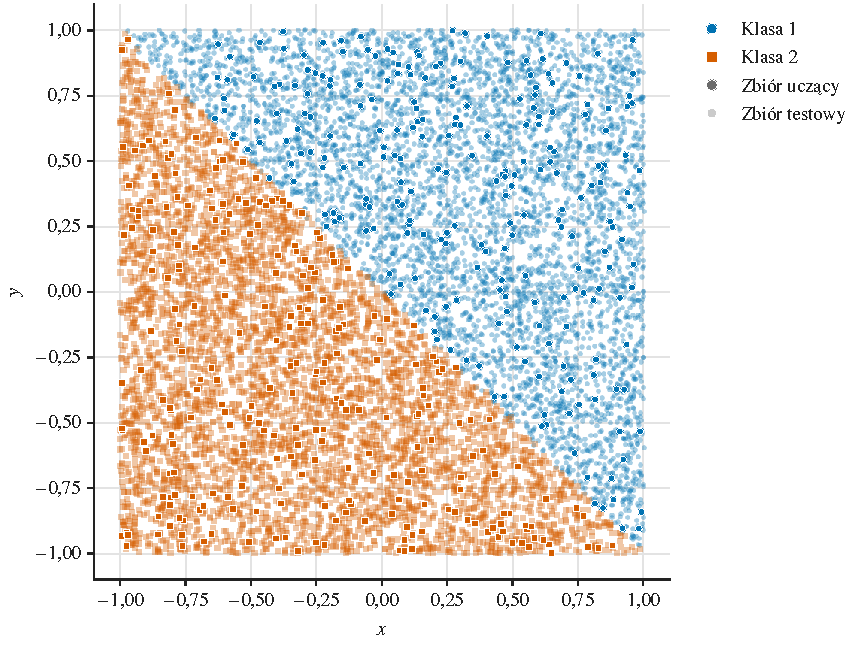
\includegraphics[width=\textwidth]{classification/showcase-simple/plots/dataset.pdf}
        \caption{\texttt{simple}}
    \end{subfigure}
    \hfill
    \begin{subfigure}[b]{0.49\textwidth}
        \centering
        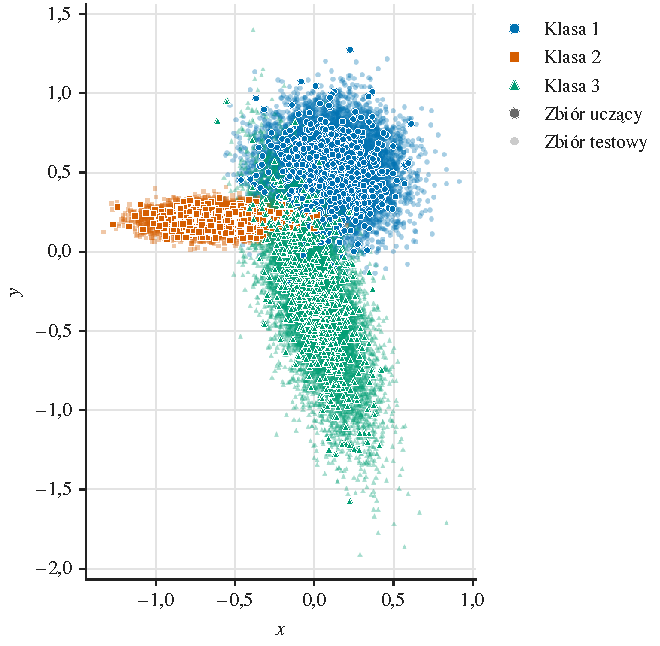
\includegraphics[width=\textwidth]{classification/showcase-three-gauss/plots/dataset.pdf}
        \caption{\texttt{three\_gauss}}
    \end{subfigure}
    \caption{Zbiory klasyfikacji: zbiór uczący o liczności \num{500} na rysunku~(a) i \num{1500} ($\num{500}$ na klasę) na rysunku~(b) oraz zbiór testowy o liczności \num{10000} na rysunku~(a) i \num{30000} na rysunku~(b).}
    \label{fig:datasets-classification}
\end{figure}

Zbiory regresji pokazano na Rysunku~\ref{fig:datasets-regression}. Funkcja w zbiorze \texttt{activation} jest monotoniczna i nasyca się na obu krańcach dziedziny, przyjmując kształt litery S. Funkcja w zbiorze \texttt{cube} ma przebieg krzywej sześciennej: między dwoma łagodnymi zagięciami jest prawie płaska, a na krańcach szybko rośnie co do wartości bezwzględnej. W obu zbiorach odpowiedzi są rzędu setek, a punkty uczące leżą blisko krzywej wyznaczonej przez zbiór testowy.

\begin{figure}[H]
    \centering
    \begin{subfigure}[b]{0.49\textwidth}
        \centering
        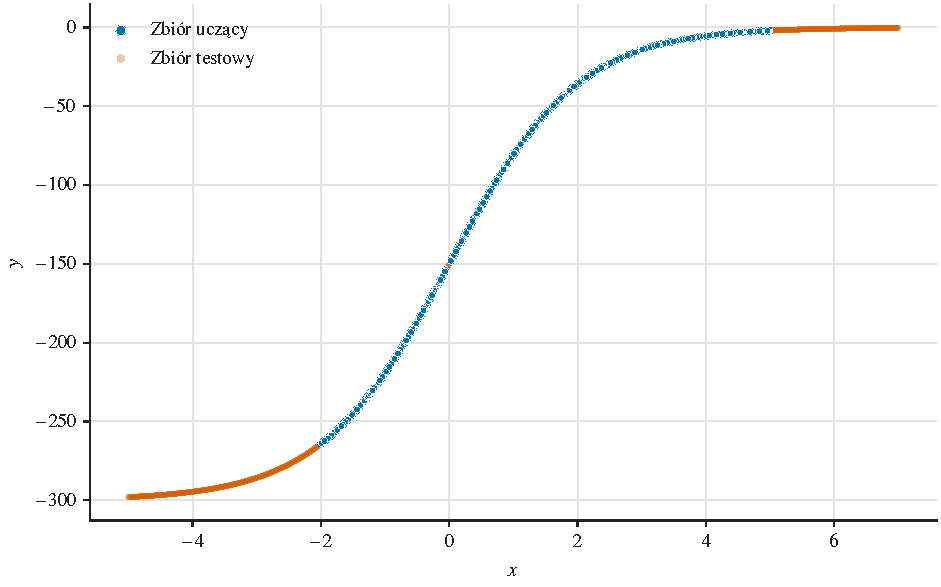
\includegraphics[width=\textwidth]{regression/showcase-activation/plots/dataset.pdf}
        \caption{\texttt{activation}}
    \end{subfigure}
    \hfill
    \begin{subfigure}[b]{0.49\textwidth}
        \centering
        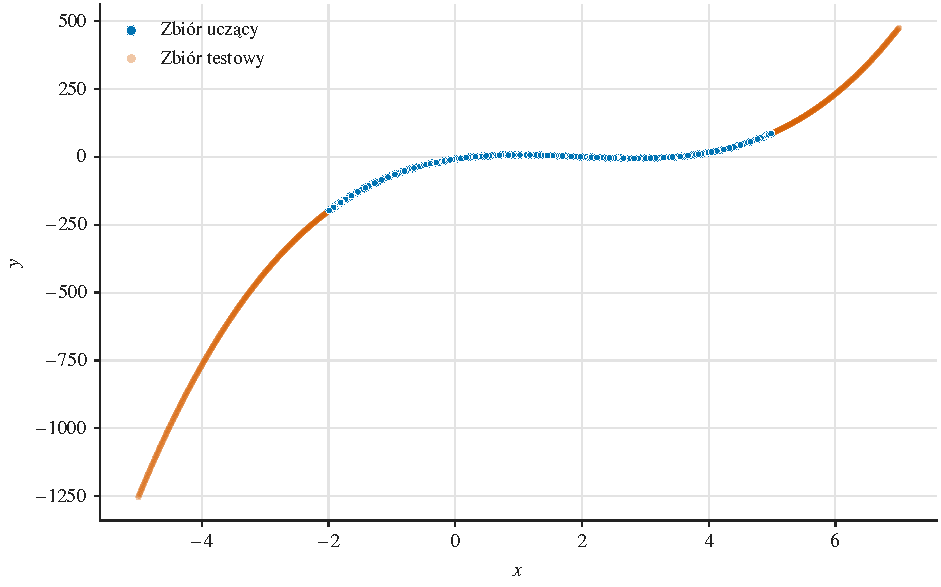
\includegraphics[width=\textwidth]{regression/showcase-cube/plots/dataset.pdf}
        \caption{\texttt{cube}}
    \end{subfigure}
    \caption{Zbiory regresji: zbiór uczący o liczności \num{500} i zbiór testowy o liczności \num{1201}.}
    \label{fig:datasets-regression}
\end{figure}

Zbiór testowy regresji jest jeden dla wszystkich liczności: \num{1201} punktów rozmieszczonych co \num{0.01} w przedziale $x \in [-5, 7]$. Wejścia zbiorów uczących leżą natomiast w przybliżeniu w przedziale $[-2, 5]$. Na części zbioru testowego model musi więc przewidywać wartości poza zakresem danych, na których był uczony, czyli ekstrapolować. Konsekwencje tego dla oceny modeli omówiono w podrozdziale~\ref{sec:methodology-metrics} i rozdziale~\ref{sec:regression}.

\subsection{Zakres badań}
\label{sec:problem-scope}

Zadanie projektowe wymaga implementacji perceptronu wielowarstwowego uczonego algorytmem propagacji wstecznej błędu z metodą stochastycznego spadku wzdłuż gradientu (ang. \textit{stochastic gradient descent}, SGD) lub jej wariantem, bez użycia bibliotek implementujących sieci neuronowe. Implementacja ma umożliwiać powtarzalne uczenie z zadanym ziarnem generatora liczb losowych oraz łatwą konfigurację liczby warstw, liczby neuronów w warstwach i obecności biasów. Wymagane są wizualizacje zbioru uczącego i wyników klasyfikacji oraz regresji, błędu w kolejnych iteracjach uczenia oraz wartości wag w kolejnych iteracjach.

Na dostarczonych zbiorach należy zbadać wpływ trzech czynników na skuteczność sieci:
\begin{itemize}
    \item funkcji aktywacji w warstwach ukrytych: funkcji sigmoidalnej i co najmniej dwóch innych, przy aktywacji wyjściowej dobranej do rodzaju zadania,
    \item liczby warstw ukrytych, od $0$ do $4$, oraz liczby neuronów w nich,
    \item funkcji straty: dwóch dla klasyfikacji i dwóch dla regresji.
\end{itemize}

Wynik uczenia zależy od losowej inicjalizacji wag i kolejności podawania próbek, więc pojedyncze uczenie nie wystarcza do porównania wariantów. Zadanie wymaga zaadresowania tego problemu, dlatego każdy wariant uczono dla wielu ziaren generatora.

Model sieci i algorytm uczenia opisano w rozdziale~\ref{sec:mlp}, a ich implementację w rozdziale~\ref{sec:implementation}. Wymagane wizualizacje przedstawiono w rozdziale~\ref{sec:showcase}, a plan badań w rozdziale~\ref{sec:methodology}.

\section{Perceptron wielowarstwowy}
\label{sec:mlp}

\subsection{Model sieci}
\label{sec:mlp-model}
% Plan (etap 4): notacja macierzowa, warstwa Z = A W + b (wiersz = próbka), bias
% opcjonalny, propagacja w przód.

\subsection{Funkcje aktywacji}
\label{sec:mlp-activations}
% Plan (etap 4): tabela sigmoid, tanh, ReLU, leaky ReLU (wzór, pochodna, zakres);
% wyjście: identity (regresja), softmax (klasyfikacja).

\subsection{Funkcje straty}
\label{sec:mlp-losses}
% Plan (etap 4): entropia krzyżowa i MSE na kodowaniu one-hot (klasyfikacja),
% MSE i MAE (regresja).

\subsection{Propagacja wsteczna}
\label{sec:mlp-backprop}
% Plan (etap 4): wzory gradientów warstwa po warstwie, skrót (P - Y)/n dla entropii
% krzyżowej z softmax, ogólny VJP softmaxu; algorytm.

\subsection{Optymalizacja}
\label{sec:mlp-optimization}
% Plan (etap 4): mini-batch SGD, momentum, Adam; tasowanie co epokę.

\subsection{Inicjalizacja wag}
\label{sec:mlp-init}
% Plan (etap 4): inicjalizacja Xaviera (sigmoid, tanh) i He (ReLU, leaky ReLU).

\section{Implementacja}
\label{sec:implementation}

\subsection{Architektura rozwiązania}
\label{sec:implementation-architecture}
% Plan (etap 5): warstwa obliczeniowa (Rust) i warstwa prezentacji (Python)
% komunikujące się przez pliki; przepływ config -> train -> artefakty -> wykresy.

\subsection{Konfiguracja eksperymentu}
\label{sec:implementation-config}
% Plan (etap 5): plik config.toml (listing, tabela sekcji i kluczy), walidacja
% z diagnostyką wskazującą linię.

\subsection{Przygotowanie danych}
\label{sec:implementation-data}
% Plan (etap 5): wczytywanie CSV, kodowanie klas, normalizacja dopasowana do zbioru
% uczącego, podzbiór i wydzielenie walidacji.

\subsection{Sieć i uczenie}
\label{sec:implementation-network}
% Plan (etap 5): warstwy jako macierze ndarray, asercje wymiarów, pętla uczenia,
% obserwator, wykrywanie dywergencji, opcjonalny early stopping.

\subsection{Powtarzalność}
\label{sec:implementation-reproducibility}
% Plan (etap 5): jedno ziarno, osobne strumienie RNG (dane, inicjalizacja, tasowanie,
% próbkowanie wag), wersja kodu w metadata.json.

\subsection{Weryfikacja poprawności}
\label{sec:implementation-verification}
% Plan (etap 5): numeryczny gradient check (różnice centralne), testy determinizmu,
% CI.

\subsection{Artefakty, wizualizacja i automatyzacja badań}
\label{sec:implementation-analysis}
% Plan (etap 5): artefakty (.npy, epochs.csv, metadata.json), wykresy w Pythonie,
% study.toml -> generate -> train -> aggregate.

\section{Wizualizacja procesu uczenia}
\label{sec:showcase}

\subsection{Klasyfikacja}
\label{sec:showcase-classification}
% Plan (etap 6): eksperyment showcase-three-gauss: zbiór, granica decyzyjna, błąd po
% iteracjach, ewolucja wag (trajektorie, normy, heatmapa), macierz pomyłek.

\subsection{Regresja}
\label{sec:showcase-regression}
% Plan (etap 6): eksperyment showcase-cube: dane i krzywa sieci, błąd po iteracjach,
% ewolucja wag.

\section{Metodyka eksperymentów}
\label{sec:methodology}

\subsection{Plan badań}
\label{sec:methodology-plan}
% Plan (etap 7): tabela 12 badań jeden-czynnik-naraz (czynnik, poziomy, zbiory),
% oś rozmiaru 100/500/1000/10000, 10 ziaren.

\subsection{Konfiguracja bazowa}
\label{sec:methodology-base}
% Plan (etap 7): tabela hiperparametrów bazy, tabela epok i iteracji na rozmiar.

\subsection{Miary jakości i statystyki}
\label{sec:methodology-metrics}
% Plan (etap 7): dokładność testowa (średnia i odchylenie), MSE testowe (mediana
% i kwartyle), MSE w zakresie i poza zakresem zbioru uczącego.

\subsection{Założenia i ograniczenia planu}
\label{sec:methodology-caveats}
% Plan (etap 7): budżet rośnie z rozmiarem, rozłączne pliki, wspólny zbiór testowy,
% jedno lr, brak early stoppingu.

\section{Wyniki klasyfikacji}
\label{sec:classification}
% Plan (etap 8): zbiory simple i three_gauss; dokładność testowa; wybór wykresów
% (heatmapy, curves, galerie) w planie etapu.

\subsection{Funkcje aktywacji}
\label{sec:classification-activations}
% Plan (etap 8): badania simple-activations i three-gauss-activations.

\subsection{Architektura sieci}
\label{sec:classification-architectures}
% Plan (etap 8): badania simple-architectures i three-gauss-architectures.

\subsection{Funkcje straty}
\label{sec:classification-losses}
% Plan (etap 8): badania simple-losses i three-gauss-losses.

\section{Wyniki regresji}
\label{sec:regression}

W rozdziale przedstawiono wyniki sześciu badań regresji, po trzy dla zbiorów \texttt{activation} i \texttt{cube}. Miarą jest MSE testowe w oryginalnej skali odpowiedzi, podawane jako mediana i kwartyle po $10$ ziarnach, osobno dla punktów w zakresie zbioru uczącego \eqref{eq:mse-inside} i poza nim \eqref{eq:mse-outside}. Błąd w zakresie mierzy dopasowanie do funkcji w obszarze danych uczących, a błąd poza zakresem zależy tylko od tego, jak sieć przedłuża swoją funkcję tam, gdzie nie widziała żadnych danych.

\subsection{Funkcje aktywacji}
\label{sec:regression-activations}

Wyniki badania funkcji aktywacji dla zbioru \texttt{activation} przedstawiono na Rysunku~\ref{fig:regression-activation-activations-heatmaps}. W zakresie zbioru uczącego najlepsza przy każdej liczności jest funkcja tanh, z medianą MSE od \num{0.0208} do \num{0.0372}. Funkcja sigmoidalna osiąga od \num{0.0319} do \num{0.156}, a ReLU i leaky ReLU od \num{0.269} do \num{2.63}. Poza zakresem różnice sięgają trzech rzędów wielkości. Mediana MSE wynosi od \num{0.600} do \num{2.33} dla funkcji tanh, od \num{38.0} do \num{120} dla funkcji sigmoidalnej i od \num{1410} do \num{2200} dla ReLU i leaky ReLU.

\begin{figure}[H]
    \centering
    \begin{subfigure}[b]{0.49\textwidth}
        \centering
        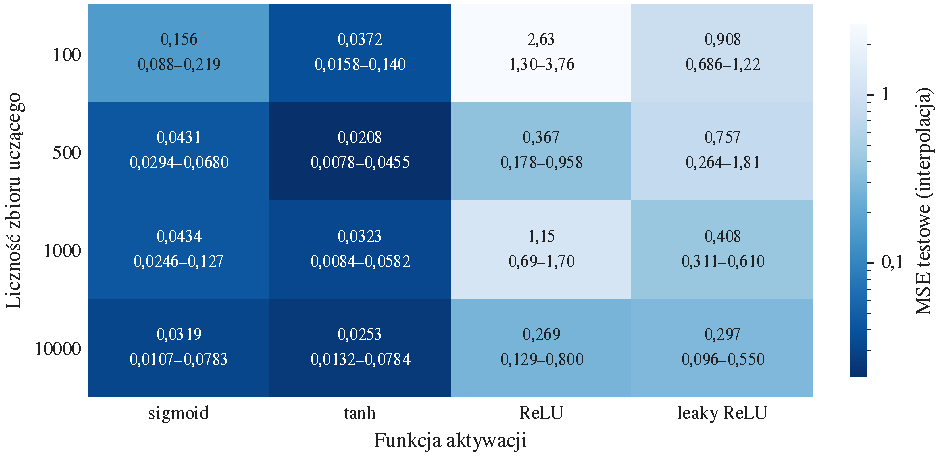
\includegraphics[width=\textwidth]{regression/activation-activations/results/heatmap_inside.pdf}
        \caption{w zakresie zbioru uczącego}
    \end{subfigure}
    \hfill
    \begin{subfigure}[b]{0.49\textwidth}
        \centering
        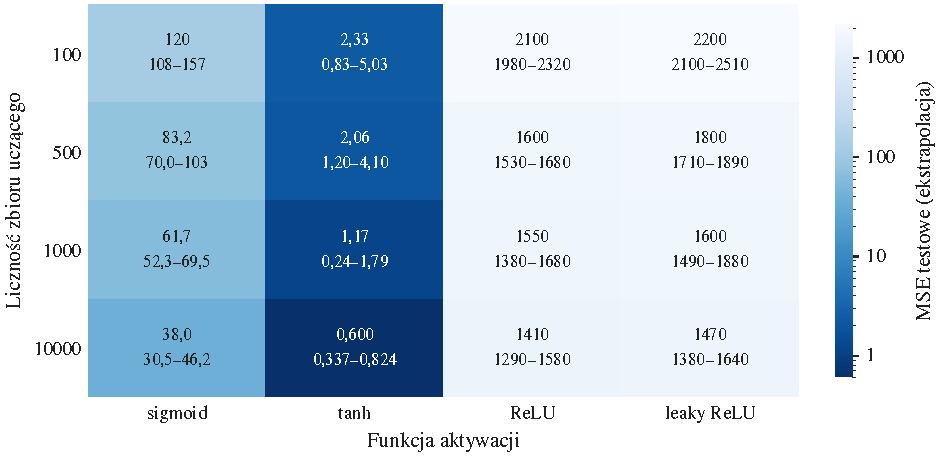
\includegraphics[width=\textwidth]{regression/activation-activations/results/heatmap_outside.pdf}
        \caption{poza zakresem zbioru uczącego}
    \end{subfigure}
    \caption{MSE testowe na zbiorze \texttt{activation} w zależności od funkcji aktywacji warstw ukrytych i liczności zbioru uczącego: mediana i kwartyle po $10$ ziarnach.}
    \label{fig:regression-activation-activations-heatmaps}
\end{figure}

Źródło tych różnic widać na Rysunku~\ref{fig:regression-activation-activations-gallery}, który dla każdej funkcji aktywacji pokazuje jedno z $10$ uczeń przy liczności \num{1000}: to, którego MSE testowe jest najbliższe medianie po ziarnach. W zakresie danych uczących wszystkie cztery sieci pokrywają się z funkcją docelową. Poza nim sieci z funkcjami tanh i sigmoidalną nasycają się tak jak funkcja docelowa, przy czym sieć z funkcją sigmoidalną na lewym krańcu dochodzi do innego poziomu. Sieci z ReLU i leaky ReLU przedłużają funkcję prostą, która coraz bardziej oddala się od nasyconej funkcji docelowej.

\begin{figure}[H]
    \centering
    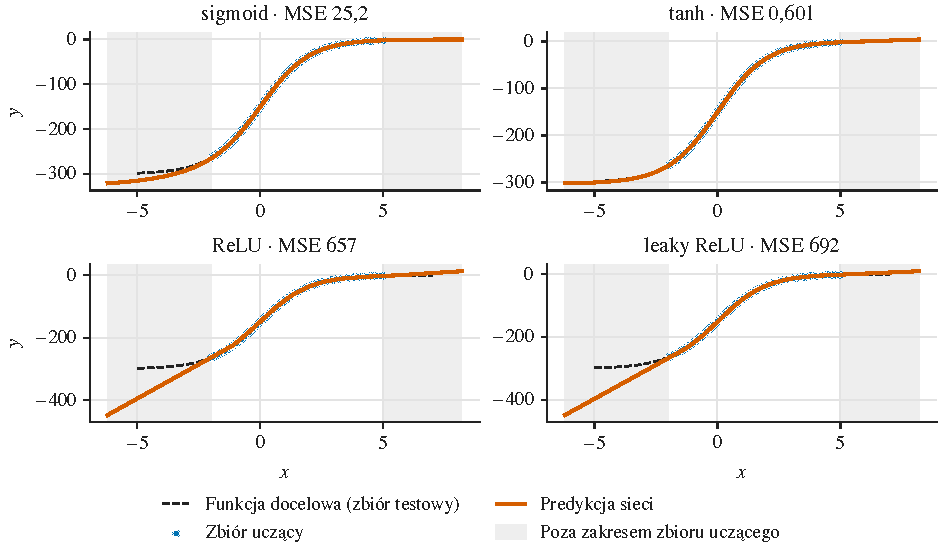
\includegraphics[width=0.9\textwidth]{regression/activation-activations/results/gallery_1000.pdf}
    \caption{Funkcja sieci na zbiorze \texttt{activation} przy liczności \num{1000} dla każdej funkcji aktywacji: uczenie o MSE testowym najbliższym medianie po ziarnach i jego MSE testowe. Szare pasy oznaczają obszar poza zakresem zbioru uczącego.}
    \label{fig:regression-activation-activations-gallery}
\end{figure}

Daleko od danych pobudzenia neuronów pierwszej warstwy ukrytej rosną co do wartości bezwzględnej liniowo z $x$. Funkcje tanh i sigmoidalna mają ograniczony zbiór wartości (Tabela~\ref{tab:activations}), więc ich wyjścia stają się stałe, a z nimi cała funkcja sieci. Sieć z funkcjami ReLU lub leaky ReLU jest funkcją kawałkami liniową, więc daleko od danych jest liniowa \cite{xu2021}. Funkcja docelowa zbioru \texttt{activation} nasyca się na obu krańcach (podrozdział~\ref{sec:problem-datasets}), dlatego przedłużenie stałe pasuje do niej, a przedłużenie liniowe nie.

Wyniki dla zbioru \texttt{cube} przedstawiono na Rysunku~\ref{fig:regression-cube-activations-heatmaps}. W zakresie zbioru uczącego przy liczności \num{100} najlepsza jest funkcja tanh (\num{0.680}), a najsłabsza funkcja sigmoidalna (\num{5.94}). Przy liczności \num{10000} kolejność się zmienia: funkcja sigmoidalna osiąga \num{0.196}, tanh \num{0.266}, a ReLU i leaky ReLU \num{0.463} i \num{0.753}. Poza zakresem wszystkie sieci mają błędy rzędu $10^{4}$--$10^{5}$. Najmniejsze ma leaky ReLU (od \num{62200} do \num{75700}), następnie ReLU (od \num{73100} do \num{82600}), tanh (od \num{83400} do \num{94500}) i funkcja sigmoidalna (od \num{89100} do \num{121000}).

\begin{figure}[H]
    \centering
    \begin{subfigure}[b]{0.49\textwidth}
        \centering
        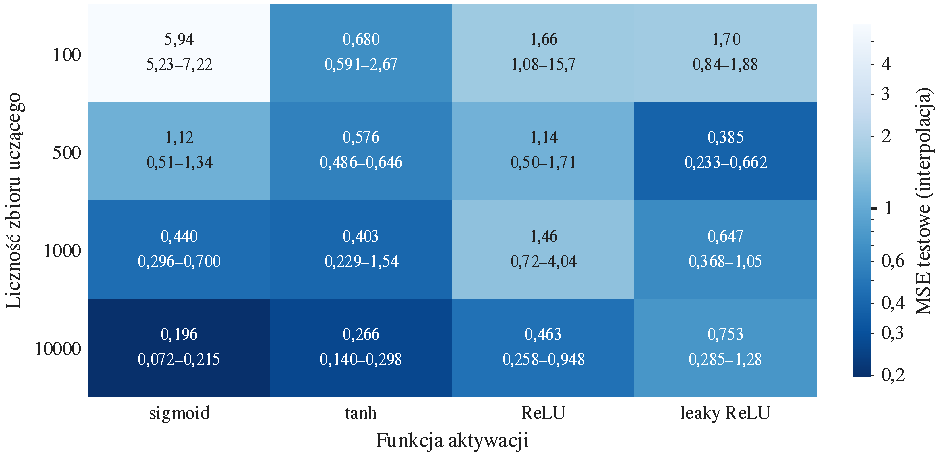
\includegraphics[width=\textwidth]{regression/cube-activations/results/heatmap_inside.pdf}
        \caption{w zakresie zbioru uczącego}
    \end{subfigure}
    \hfill
    \begin{subfigure}[b]{0.49\textwidth}
        \centering
        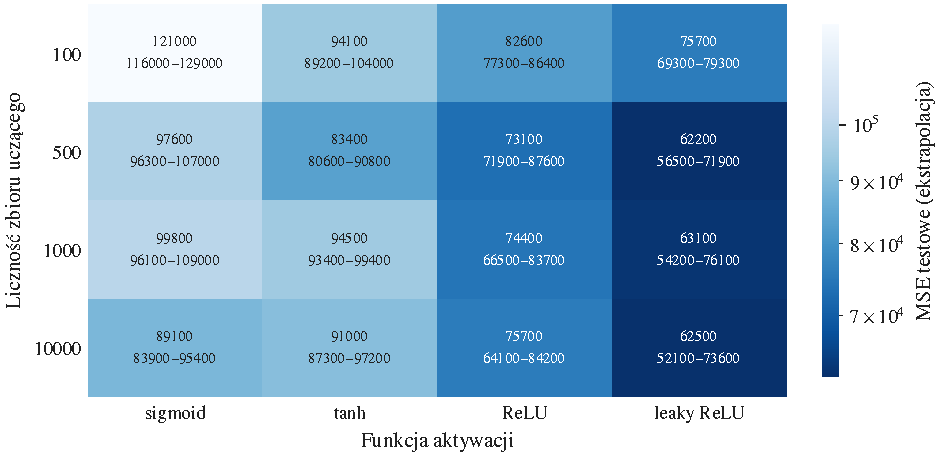
\includegraphics[width=\textwidth]{regression/cube-activations/results/heatmap_outside.pdf}
        \caption{poza zakresem zbioru uczącego}
    \end{subfigure}
    \caption{MSE testowe na zbiorze \texttt{cube} w zależności od funkcji aktywacji warstw ukrytych i liczności zbioru uczącego: mediana i kwartyle po $10$ ziarnach.}
    \label{fig:regression-cube-activations-heatmaps}
\end{figure}

Funkcja docelowa zbioru \texttt{cube} na krańcach szybko rośnie co do wartości bezwzględnej, szybciej niż jakakolwiek prosta. Żadna z badanych sieci nie może więc jej przedłużyć, a ranking poza zakresem mówi tylko, której sieci przedłużenie najmniej odbiega od funkcji docelowej. Przedłużenie liniowe sieci z ReLU i leaky ReLU podąża za wzrostem funkcji dłużej niż przedłużenie stałe sieci z funkcjami tanh i sigmoidalną.

\subsection{Architektura sieci}
\label{sec:regression-architectures}

Wyniki badania architektur dla zbioru \texttt{activation} przedstawiono na Rysunku~\ref{fig:regression-activation-architectures-heatmaps}. Sieć bez warstw ukrytych, czyli model liniowy, ma w zakresie zbioru uczącego medianę MSE od \num{693} do \num{708}. Sieci z warstwami ukrytymi osiągają od \num{0.00225} do \num{0.470}, czyli co najmniej o trzy rzędy wielkości mniej. Ich kolejność zmienia się z licznością, a kwartyle są szerokie, więc nie wskazują jednej najlepszej architektury. Poza zakresem sieci z jedną warstwą ukrytą mają medianę MSE od \num{4.55} do \num{54.4}, a sieci z co najmniej dwiema warstwami od \num{0.492} do \num{10.3}. U sieci 64-64 i 64-64-64-64 mediana mieści się przy każdej liczności w przedziale od \num{0.984} do \num{1.77}. Największe błędy wśród sieci z warstwami ukrytymi ma jedna warstwa z $64$ neuronami, od \num{18.9} do \num{54.4}. Sieć bez warstw ukrytych ma poza zakresem ponad \num{3900}.

\begin{figure}[H]
    \centering
    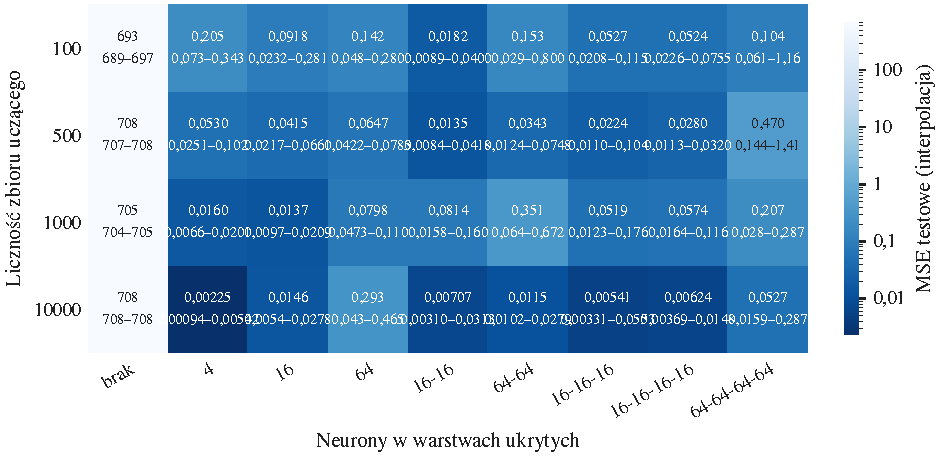
\includegraphics[width=\textwidth]{regression/activation-architectures/results/heatmap_inside.pdf}

    \vspace{1ex}
    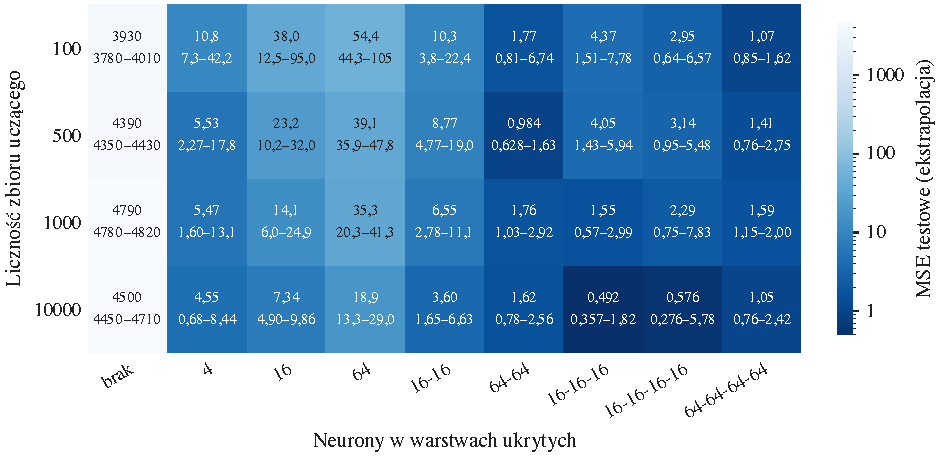
\includegraphics[width=\textwidth]{regression/activation-architectures/results/heatmap_outside.pdf}
    \caption{MSE testowe na zbiorze \texttt{activation} w zależności od architektury i liczności zbioru uczącego: mediana i kwartyle po $10$ ziarnach. Górny wykres: w zakresie zbioru uczącego. Dolny wykres: poza zakresem zbioru uczącego.}
    \label{fig:regression-activation-architectures-heatmaps}
\end{figure}

Wyniki dla zbioru \texttt{cube} przedstawiono na Rysunku~\ref{fig:regression-cube-architectures-heatmaps}. Model liniowy ma w zakresie zbioru uczącego medianę MSE od \num{889} do \num{1010}. Przy każdej liczności każda sieć z co najmniej dwiema warstwami ukrytymi jest lepsza od każdej sieci z jedną warstwą. Przy liczności \num{100} mediany wynoszą od \num{0.930} do \num{1.96} wobec od \num{11.6} do \num{30.9}, a przy liczności \num{10000} od \num{0.115} do \num{0.772} wobec od \num{1.12} do \num{1.49}. Poza zakresem najmniejszy błąd ma jedna warstwa z $64$ neuronami (od \num{59800} do \num{90400}), a największy spośród sieci z warstwami ukrytymi sieć 64-64-64-64 (od \num{137000} do \num{161000}).

\begin{figure}[H]
    \centering
    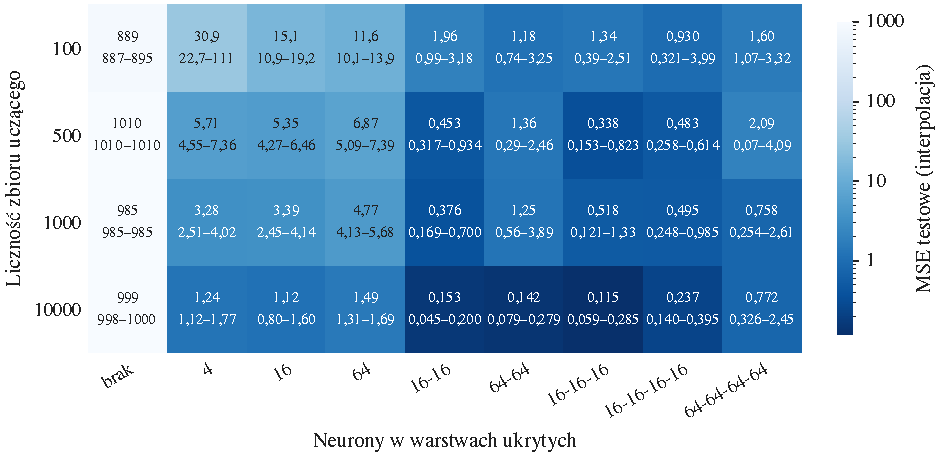
\includegraphics[width=\textwidth]{regression/cube-architectures/results/heatmap_inside.pdf}

    \vspace{1ex}
    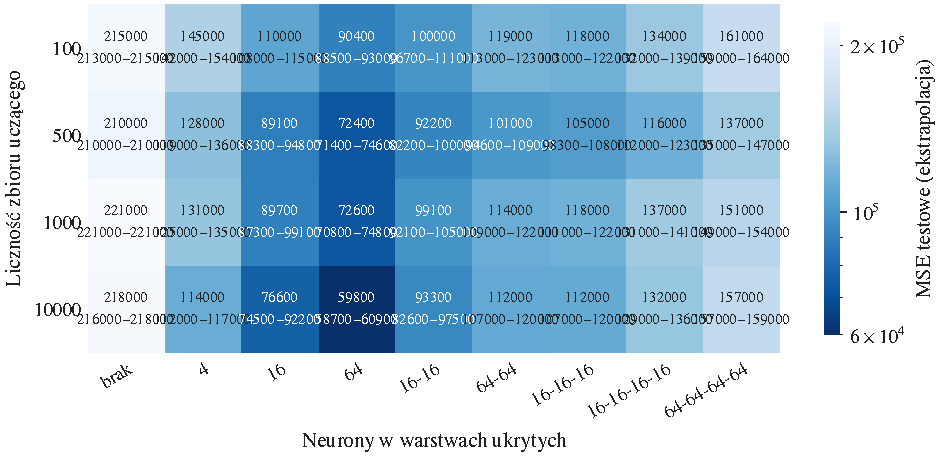
\includegraphics[width=\textwidth]{regression/cube-architectures/results/heatmap_outside.pdf}
    \caption{MSE testowe na zbiorze \texttt{cube} w zależności od architektury i liczności zbioru uczącego: mediana i kwartyle po $10$ ziarnach. Górny wykres: w zakresie zbioru uczącego. Dolny wykres: poza zakresem zbioru uczącego.}
    \label{fig:regression-cube-architectures-heatmaps}
\end{figure}

Funkcje sieci o różnych architekturach przy liczności \num{1000} pokazano na Rysunku~\ref{fig:regression-cube-architectures-gallery}, w tej samej postaci co na Rysunku~\ref{fig:regression-activation-activations-gallery}. Model liniowy nie dopasowuje się do funkcji nawet w zakresie danych uczących. Pozostałe sieci pokrywają się z funkcją docelową w zakresie danych, a poza nim wypłaszczają się, podczas gdy funkcja docelowa rośnie dalej. Sieci głębokie wypłaszczają się najszybciej, a sieć z jedną warstwą $64$ neuronów przedłuża wzrost najdłużej, stąd jej najmniejszy błąd poza zakresem.

\begin{figure}[H]
    \centering
    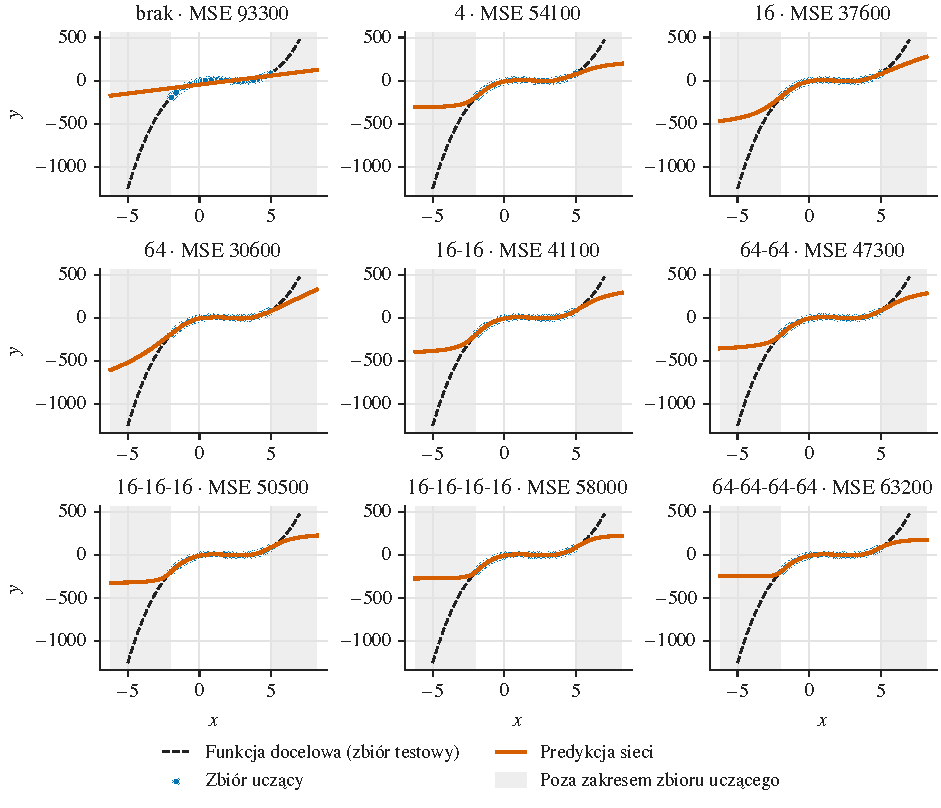
\includegraphics[width=0.9\textwidth]{regression/cube-architectures/results/gallery_1000.pdf}
    \caption{Funkcja sieci na zbiorze \texttt{cube} przy liczności \num{1000} dla każdej architektury: uczenie o MSE testowym najbliższym medianie po ziarnach i jego MSE testowe. Szare pasy oznaczają obszar poza zakresem zbioru uczącego.}
    \label{fig:regression-cube-architectures-gallery}
\end{figure}

\subsection{Funkcje straty}
\label{sec:regression-losses}

Wyniki badania funkcji straty przedstawiono na Rysunkach~\ref{fig:regression-activation-losses-heatmaps} i~\ref{fig:regression-cube-losses-heatmaps}. Sieć uczona na MSE jest w zakresie zbioru uczącego wyraźnie lepsza od sieci uczonej na MAE. Mediana MSE sieci uczonej na MAE jest od \num{14.6} do \num{22.6} razy większa w zbiorze \texttt{activation} i od \num{5.91} do \num{8.21} razy większa w zbiorze \texttt{cube}. Poza zakresem sieć uczona na MSE jest lepsza w zbiorze \texttt{activation} (od \num{2.81} do \num{5.66} razy), a w zbiorze \texttt{cube} stosunek median wynosi od \num{0.93} do \num{1.10}, więc nie ma systematycznej różnicy.

\begin{figure}[H]
    \centering
    \begin{subfigure}[b]{0.49\textwidth}
        \centering
        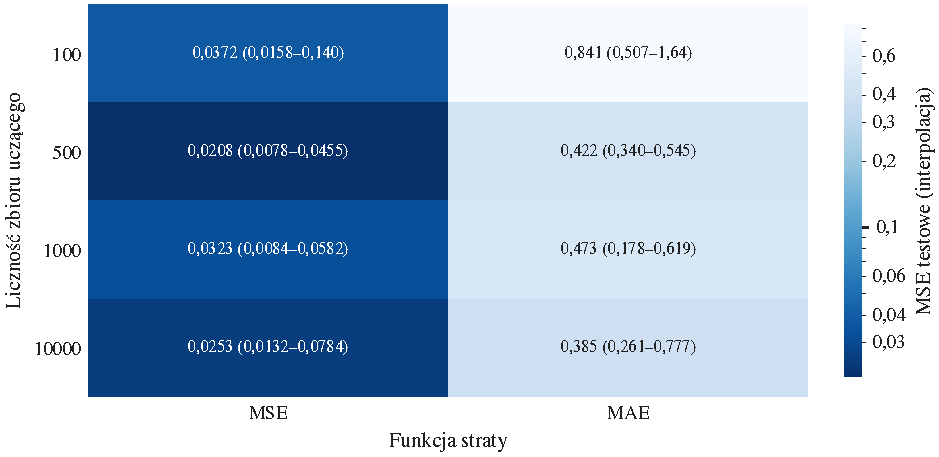
\includegraphics[width=\textwidth]{regression/activation-losses/results/heatmap_inside.pdf}
        \caption{w zakresie zbioru uczącego}
    \end{subfigure}
    \hfill
    \begin{subfigure}[b]{0.49\textwidth}
        \centering
        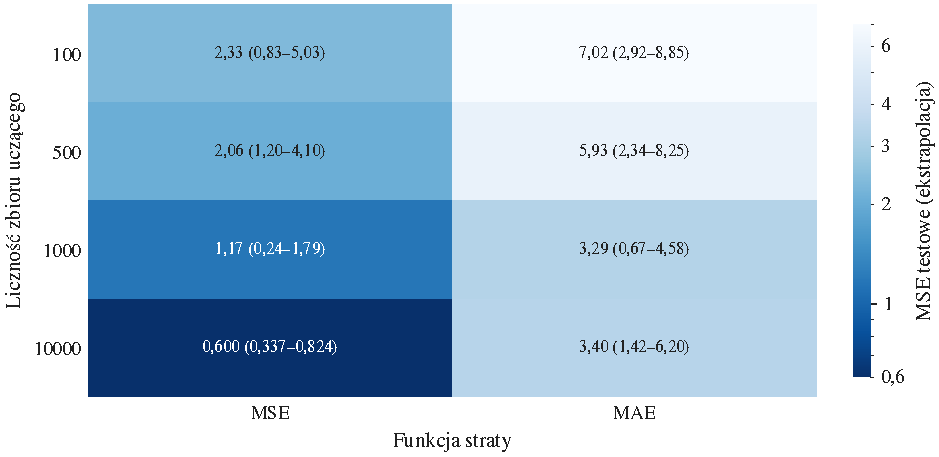
\includegraphics[width=\textwidth]{regression/activation-losses/results/heatmap_outside.pdf}
        \caption{poza zakresem zbioru uczącego}
    \end{subfigure}
    \caption{MSE testowe na zbiorze \texttt{activation} w zależności od funkcji straty i liczności zbioru uczącego: mediana i kwartyle po $10$ ziarnach.}
    \label{fig:regression-activation-losses-heatmaps}
\end{figure}

\begin{figure}[H]
    \centering
    \begin{subfigure}[b]{0.49\textwidth}
        \centering
        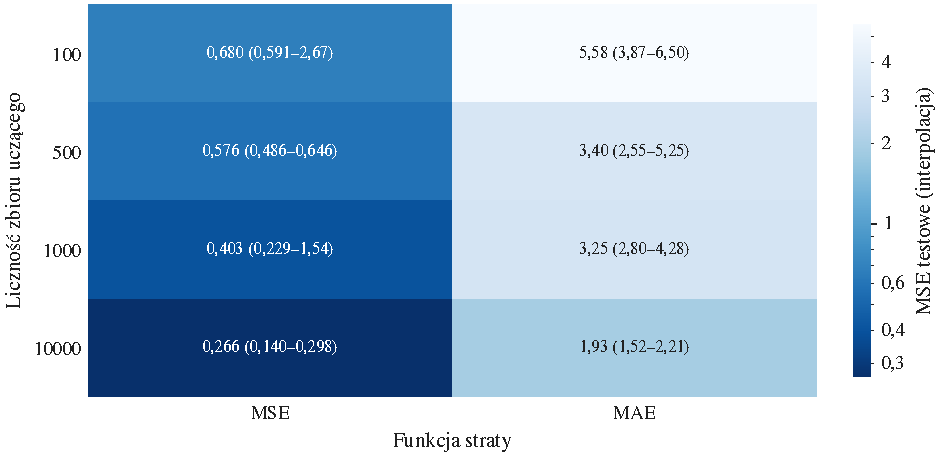
\includegraphics[width=\textwidth]{regression/cube-losses/results/heatmap_inside.pdf}
        \caption{w zakresie zbioru uczącego}
    \end{subfigure}
    \hfill
    \begin{subfigure}[b]{0.49\textwidth}
        \centering
        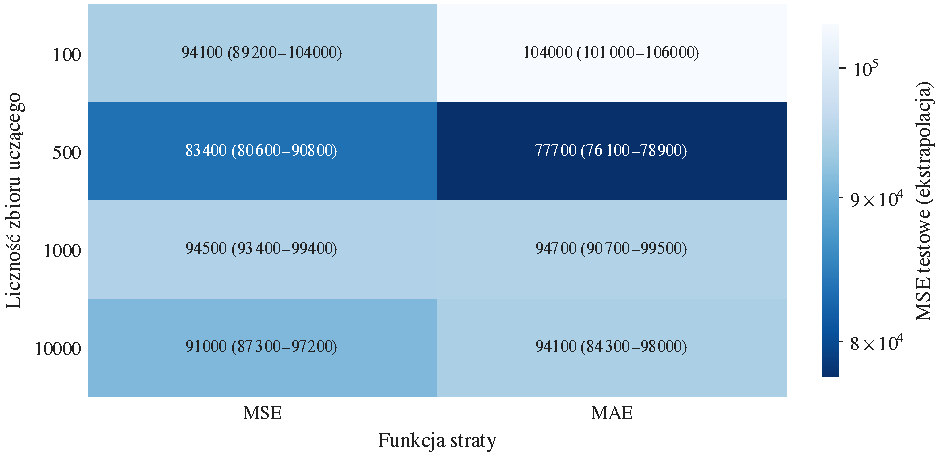
\includegraphics[width=\textwidth]{regression/cube-losses/results/heatmap_outside.pdf}
        \caption{poza zakresem zbioru uczącego}
    \end{subfigure}
    \caption{MSE testowe na zbiorze \texttt{cube} w zależności od funkcji straty i liczności zbioru uczącego: mediana i kwartyle po $10$ ziarnach.}
    \label{fig:regression-cube-losses-heatmaps}
\end{figure}

Miara MSE z definicji sprzyja sieci, która ją minimalizuje. Dlatego porównano też średni błąd bezwzględny na całym zbiorze testowym. W zbiorze \texttt{activation} sieć uczona na MSE jest lepsza także w tej mierze, z medianą od \num{0.374} do \num{0.619} wobec od \num{0.763} do \num{1.27} dla sieci uczonej na MAE. W zbiorze \texttt{cube} błąd bezwzględny na całym zbiorze testowym zależy głównie od punktów poza zakresem, a mediany obu sieci różnią się o co najwyżej \qty{8}{\percent}.

Sieć uczona na MAE ma również większe MSE na zbiorze uczącym, od \num{14.3} do \num{21.6} razy w zbiorze \texttt{activation} i od \num{7.08} do \num{8.30} razy w zbiorze \texttt{cube}. Gorszy wynik w zakresie danych wynika więc z mniej dokładnego dopasowania do zbioru uczącego, a nie z gorszego uogólniania. Zaletą MAE jest mniejsza wrażliwość na pojedyncze duże błędy, np. punkty odstające \cite[rozdz.~1.5.5]{bishop2006}. W badanych zbiorach punkty uczące leżą blisko funkcji docelowej (podrozdział~\ref{sec:problem-datasets}), więc ta zaleta nie ma okazji się ujawnić.

\section{Analiza przekrojowa}
\label{sec:cross}

\subsection{Rozmiar zbioru uczącego i przeuczenie}
\label{sec:cross-size}
% Plan (etap 10): luka między dokładnością uczącą a testową, pojemność sieci a liczba
% próbek, ekstrapolacja nie poprawia się z liczbą danych.

\subsection{Powtarzalność między ziarnami}
\label{sec:cross-seeds}
% Plan (etap 10): rozrzut wyników między 10 ziarnami w klasyfikacji i regresji,
% brak dywergencji.

\section{Podsumowanie i wnioski}
\label{sec:conclusions}

\subsection{Wnioski}
\label{sec:conclusions-findings}
% Plan (etap 11): najważniejsze wnioski z rozdziałów wyników, tylko efekty większe
% niż rozrzut między ziarnami jako mocne.

\subsection{Ograniczenia i dalsze prace}
\label{sec:conclusions-limitations}
% Plan (etap 11): badanie jeden-czynnik-naraz, brak early stoppingu, jedno lr,
% MAE oceniane MSE.


%----------------------------------------------------------------------
\newpage
\printbibliography[heading=bibintoc]

%----------------------------------------------------------------------
\appendix
\section{Odtworzenie wyników}
\label{app:reproduction}

Do odtworzenia wyników potrzebne są kompilator języka Rust w wersji 1.88.0, wskazanej w pliku \texttt{rust-toolchain.toml}, oraz Python w wersji co najmniej 3.13 z menedżerem pakietów \texttt{uv}, który instaluje zależności w wersjach zapisanych w pliku \texttt{uv.lock}. Ścieżki w plikach konfiguracyjnych są względne, dlatego polecenia uruchamia się z katalogu głównego repozytorium. Polecenia przedstawiono na Listingu~\ref{lst:reproduction}.

\begin{code}
\begin{Verbatim}[fontsize=\small]
# zbudowanie programu i instalacja zależności Pythona
cargo build --release --manifest-path src/compute/Cargo.toml
uv sync --project src/analysis

# eksperyment pokazowy: uczenie i wykresy
cargo run --release --manifest-path src/compute/Cargo.toml -- \
    train data/experiments/classification/showcase-three-gauss
uv run --project src/analysis src/analysis/main.py \
    plot data/experiments/classification/showcase-three-gauss

# jedno badanie: eksperymenty, uczenie, zestawienie wyników
cargo run --release --manifest-path src/compute/Cargo.toml -- \
    generate data/experiments/classification/simple-activations
cargo run --release --manifest-path src/compute/Cargo.toml -- \
    train data/experiments/classification/simple-activations
uv run --project src/analysis src/analysis/main.py \
    aggregate data/experiments/classification/simple-activations --plot-runs

# wszystkie badania części pierwszej (PowerShell 7)
pwsh -File scripts/run-studies.ps1
\end{Verbatim}
    \caption{Polecenia odtwarzające wyniki, uruchamiane z katalogu głównego repozytorium.}
    \label{lst:reproduction}
\end{code}

Konfiguracje i wyniki znajdują się w następujących miejscach:
\begin{itemize}
    \item konfiguracje eksperymentów pokazowych:\newline \texttt{data/experiments/<zadanie>/showcase-<zbiór>/config.toml},
    \item konfiguracje badań:\newline \texttt{data/experiments/<zadanie>/<zbiór>-<czynnik>/study.toml},
    \item wykresy eksperymentów pokazowych: katalog \texttt{plots/} eksperymentu,
    \item zestawienia badań: katalog \texttt{results/} badania.
\end{itemize}
Katalog \texttt{<zadanie>} to \texttt{classification} albo \texttt{regression}. Eksperymenty pokazowe używają ziarna $1$, a badania ziaren od $1$ do $10$.


\end{document}